% Figure 1 — Soma-Field Architecture: Body–Brain Coupling Diagram
% Compile: lualatex fig1_architecture.tex
% Produces fig1_architecture.pdf
%
% Three-layer stack: Brainstem / Limbic (soma-field W) / PFC
% With bidirectional coupling arrows and interoceptive body input

\documentclass[tikz, border=4pt]{standalone}
\usepackage{tikz}
\usetikzlibrary{arrows.meta, positioning, shapes.geometric, fit, backgrounds}

\begin{document}
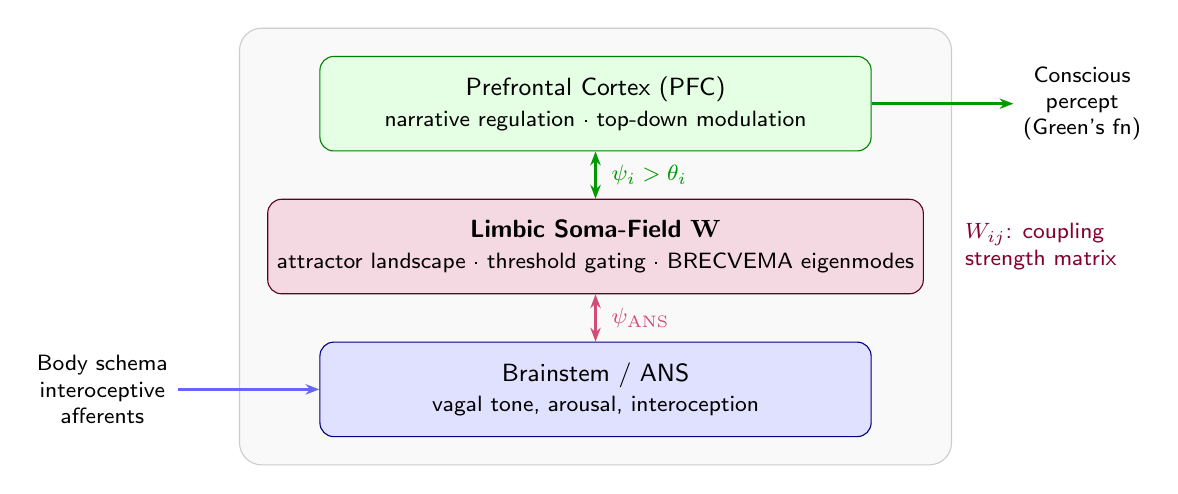
\begin{tikzpicture}[
  layer/.style   = {rectangle, rounded corners=5pt, minimum width=7cm,
                    minimum height=1.2cm, align=center, font=\sffamily\small},
  arrow/.style   = {-{Stealth[length=5pt]}, line width=1pt},
  darrow/.style  = {{Stealth[length=5pt]}-{Stealth[length=5pt]}, line width=1pt},
  node distance  = 0.6cm
]

% ── Layers (bottom → top) ────────────────────────────────────────────────────
\node[layer, fill=blue!12, draw=blue!50!black]
  (bs) {Brainstem / ANS\\\footnotesize{vagal tone, arousal, interoception}};

\node[layer, fill=purple!15, draw=purple!50!black, above=of bs]
  (lim) {\textbf{Limbic Soma-Field} $\mathbf{W}$\\\footnotesize{attractor landscape · threshold gating · BRECVEMA eigenmodes}};

\node[layer, fill=green!10, draw=green!50!black, above=of lim]
  (pfc) {Prefrontal Cortex (PFC)\\\footnotesize{narrative regulation · top-down modulation}};

% ── Body input (left side) ───────────────────────────────────────────────────
\node[left=1.8cm of bs, align=center, font=\sffamily\footnotesize]
  (body) {Body schema\\interoceptive\\afferents};
\draw[arrow, blue!60] (body.east) -- (bs.west);

% ── Inter-layer arrows ───────────────────────────────────────────────────────
\draw[darrow, purple!70] (bs.north) -- (lim.south)
  node[midway, right=2pt, font=\sffamily\footnotesize] {$\psi_\mathrm{ANS}$};

\draw[darrow, green!60!black] (lim.north) -- (pfc.south)
  node[midway, right=2pt, font=\sffamily\footnotesize] {$\psi_i > \theta_i$};

% ── Output (right side) ──────────────────────────────────────────────────────
\node[right=1.8cm of pfc, align=center, font=\sffamily\footnotesize]
  (out) {Conscious\\percept\\(Green's fn)};
\draw[arrow, green!60!black] (pfc.east) -- (out.west);

% ── Coupling constant label ───────────────────────────────────────────────────
\node[right=0.4cm of lim, align=left, font=\sffamily\footnotesize, text=purple!70!black]
  (wlabel) {$W_{ij}$: coupling\\strength matrix};

% ── Background box ───────────────────────────────────────────────────────────
\begin{scope}[on background layer]
  \node[fit=(bs)(lim)(pfc), fill=gray!5, rounded corners=8pt, draw=gray!40,
        inner sep=10pt] {};
\end{scope}

\end{tikzpicture}
\end{document}
